% TODO relire et modifier les warnings
\newpage
\subsubsection{Les interfaces du système}
Cette section décrit les entrées et sorties dites « logiques » et « physiques » du SàE.
En effet, nous différencions dans cette étude deux grands types d'entrées/sorties : 
\begin{itemize}
  \item Celles dites de haut niveau (dites aussi logiques) qui décrivent les données échangées et événements entre Utilisateur, le SàE et E\_TableauDeBord. Les entrées/sorties logiques seront décrites à la section \ref{interfaces_logiques}.
  \item Celles dites de bas niveau (dites aussi physiques) qui sont les entrées/sorties réellement échangées entre le SàE et E\_TableauDeBord. Les entrées/sorties physiques 
  (ou bas niveau) seront décrites au chapitre \ref{interfaces_physiques}.
\end{itemize}

\paragraph{Les interfaces logiques}
\label{interfaces_logiques}
Le SàE est constitué d'une application Android nommée {\nomApplication} et un programme embarqué sur la Raspberry Pi nommé {\nomLogiciel}. 

\vspace{6pt}

La figure \ref{schema_contexte_log} présente le contexte en faisant figurer les entrées/sorties logiques. Cette représentation du contexte est sous la forme d'un diagramme de communication UML. Les éléments soulignés correspondent à des ensembles de messages qui vont être détaillés. \\

\begin{figure}[ht] 
    \centering
    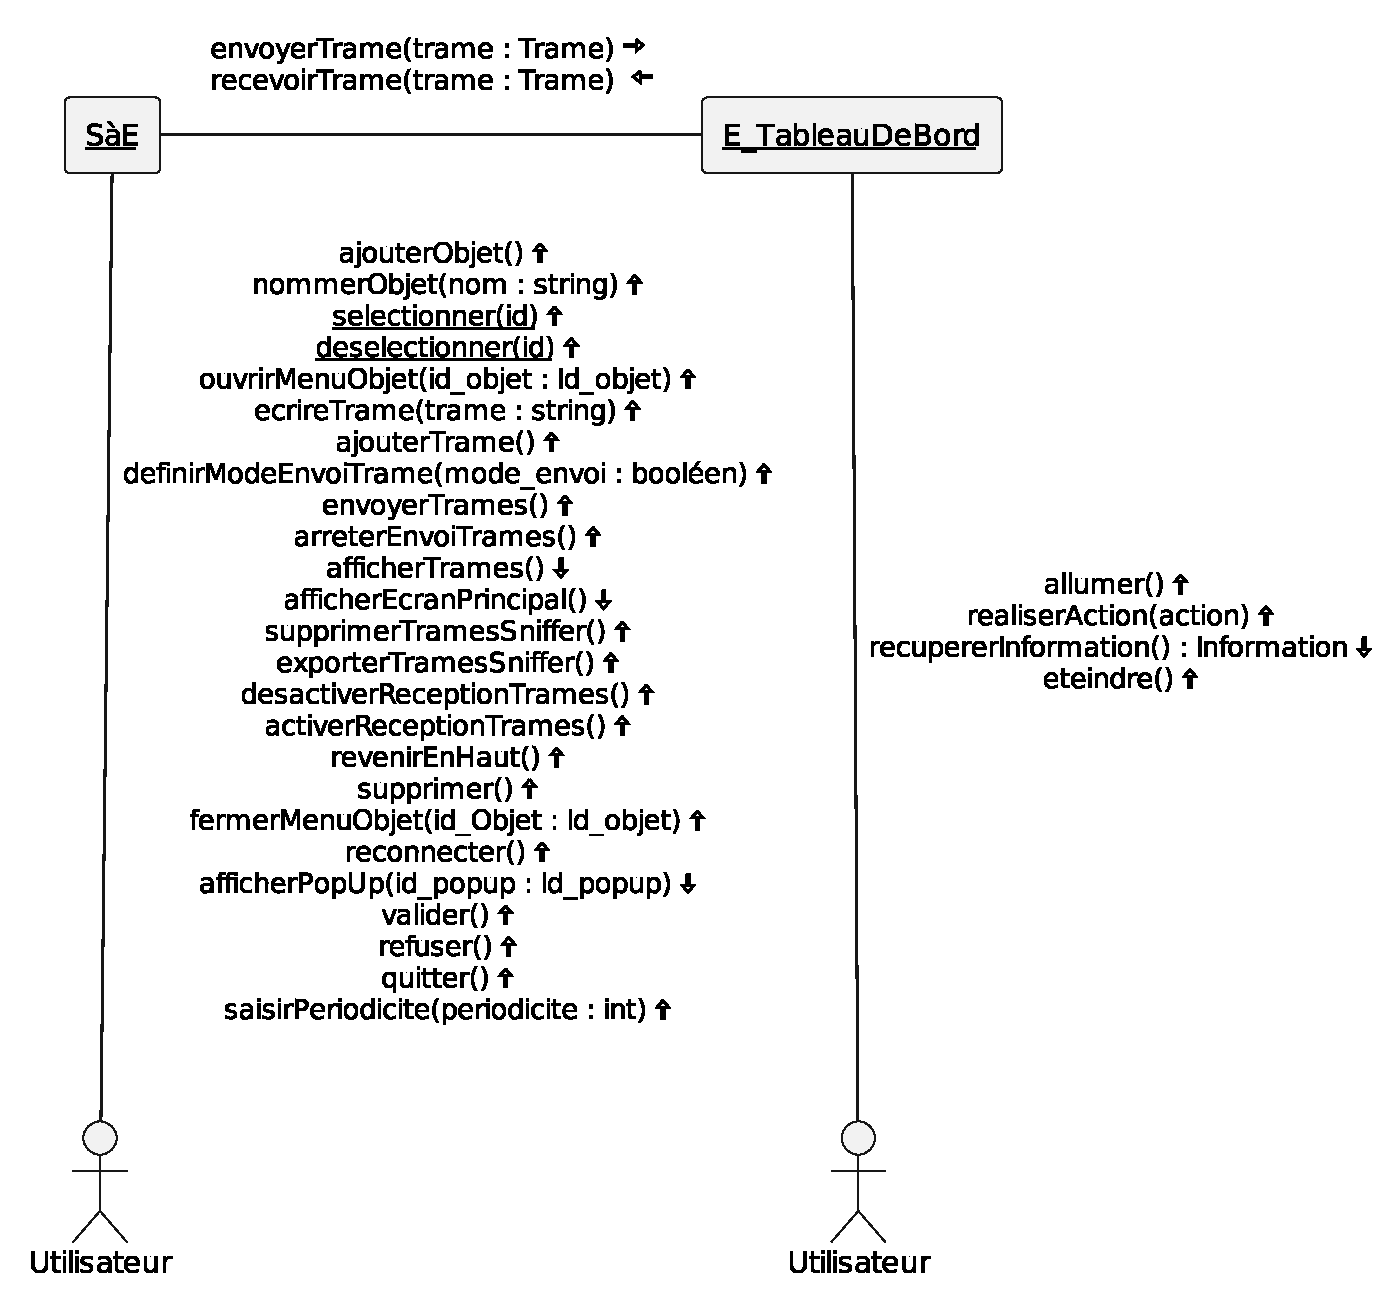
\includegraphics[width=12cm]{../schemas/contexte_log}
    \caption{Contexte logique représenté par un\\diagramme de communication UML}
    \label{schema_contexte_log}
\end{figure}

\newpage

\paragraph{Les interfaces avec les acteurs} 
L'acteur Utilisateur est en contact direct avec le SàE et Tableau de Bord. Les entrées et sorties entre Utilisateur et le SàE font référence aux fonctionnalités présentes sur l'IHM. Ces fonctionnalités sont décrites en détails dans la partie Exigences spécifiques (cf. section \ref{exigences_specifiques}). \\

Les listes d'objets et de trames mentionnées dans les descriptions suivantes sont initialement vides lors du premier lancement de l'application, mais elles sont affichées sur l'IHM. Nous allons maintenant détailler ces entrées et sorties logiques.

\vspace{-1cm}
\subparagraph{En provenance de Utilisateur}
\vspace{1cm}
\mbox{}\\

\textbf{Vers le SàE :} \vspace{0.2cm}\\ %SUBSUBPARAGRAPHE ?
\textbf{ajouterObjet()} --- Utilisateur ajoute un nouvel objet, un pop-up s'affiche ensuite pour nommer l'objet et valider l'ajout. \\
\textbf{nommerObjet(nom : string) } --- Utilisateur nomme l'objet créé dans le pop-up qui s'est affiché. Une validation est attendue. \\
\textbf{ \underline{selectionner(id)}} : 
\begin{itemize}
    \item \textbf{selectionnerObjet(id\_objet : Id\_objet)} --- Utilisateur sélectionne un objet d'ID id\_objet, il se grise ensuite. 
    \item \textbf{selectionnerTrame(id\_trame : Id\_trame)} --- Utilisateur sélectionne une trame d'ID id\_trame, elle se grise ensuite. 
\end{itemize}
\textbf{ \underline{deselectionner(id)}} : 
\begin{itemize}
    \item \textbf{deselectionnerObjet(id\_objet : Id\_objet)} --- Utilisateur désélectionne un objet d'ID id\_objet, il se dégrise ensuite. 
    \item \textbf{deselectionnerTrame(id\_trame : Id\_trame)} --- Utilisateur désélectionne une trame d'ID id\_trame, elle se dégrise ensuite. Lorsqu'il quitte le {\guillemotleft} Mode Envoi {\guillemotright}, les trames se désélectionnent automatiquement. 
\end{itemize}
\textbf{ouvrirMenuObjet(id\_objet : Id\_objet)} --- Utilisateur ouvre le menu déroulant d'un objet d'ID id\_objet. \\
\textbf{ecrireTrame(trame : string)} --- Utilisateur écrit une trame dans le menu déroulé d'un objet, le format de la trame est détaillé dans le dictionnaire de domaine (section \ref{dictionnaire}). \\
\textbf{ajouterTrame()} --- Utilisateur ajoute la trame écrite, un pop-up s'affiche pour définir le Mode Envoi de la trame.\\
\textbf{definirModeEnvoiTrame(mode\_envoi : booléen)} --- Utilisateur définit un Mode Envoi pour la trame à ajouter. Si vrai, l'envoi est ponctuel. Si faux, l'envoi est cyclique. Une validation est attendue. \\
\textbf{envoyerTrames()} --- Utilisateur demande à envoyer la ou les trames préalablement ajoutées(s) et sélectionnée(s). L'application {\nomApplication} passe alors en {\guillemotleft} Mode Envoi {\guillemotright}, et Utilisateur ne peut plus supprimer de trames ou ajouter d'objets. L'envoi des trames continue même si Utilisateur met en veille l'application {\nomApplication}.  \\
\textbf{arreterEnvoiTrames()} --- Utilisateur arrête l'envoi des trames. L'application {\nomApplication} quitte le {\guillemotleft} Mode Envoi {\guillemotright} et Utilisateur a de nouveau accès aux fonctionnalités de suppression d'élément et d'ajout d'objet.\\
\textbf{supprimerTramesSniffer()} --- Utilisateur supprime l'ensemble des trames affichées dans le sniffer. \\
\textbf{exporterTramesSniffer()} --- Utilisateur demande à exporter l'ensemble des trames affichées dans le sniffer dans un fichier de logs (voir section \ref{dictionnaire}). \\
\textbf{desactiverReceptionTrames()} --- Utilisateur désactive la réception de trames, le SàE ne va plus afficher les trames en provenance de Tableau de Bord sur l'IHM. \\
\textbf{activerReceptionTrames()} --- Utilisateur demande à activer la réception des trames, L'application {\nomApplication} affiche les trames en provenance de Tableau de Bord sur l'IHM. La reception des trames continue même si Utilisateur met en veille l'application {\nomApplication}. \\
\textbf{revenirEnHaut()} --- Utilisateur revient en haut du fil de trames affichées dans le sniffer. \\
\textbf{supprimer()} --- Utilisateur supprime les trames et objets sélectionnés. Si Utilisateur a sélectionné un ou plusieurs objets, les trames ajoutées dans le menu de ces objets seront aussi supprimées. \\
Un pop-up s'affiche pour confirmer ou non la suppression. \\
\textbf{fermerMenuObjet(id\_objet : Id\_objet)} --- Utilisateur ferme le menu précédemment ouvert d'un objet d'ID id\_objet. \\
\textbf{reconnecter()} --- Utilisateur demande à reconnecter l'application {\nomApplication} au programme {\nomLogiciel}, un pop-up s'affiche et une validation est demandée. \\
\textbf{valider()} --- Utilisateur choisit de valider son action lorsque qu'un pop-up s'affiche. \\
\textbf{refuser()} --- Utilisateur choisit de refuser de réaliser son action lorsque qu'un pop-up s'affiche.\\
\textbf{quitter()} --- Utilisateur quitte l'application {\nomApplication}. \\
\textbf{saisirPeriodicite(periodicite : int)} --- Utilisateur saisit la périodicité de la trame qu'il veut envoyer en mode cyclique. \\
\textbf{demarrer\_SSH()} --- Utilisateur démarre le programme {\nomApplication}. Le démarrage s'effectue en ligne de commande via une connexionn SSH à la Raspberry Pi. \\
\textbf{quitter\_SSH()} --- Utilisateur quitte le programme {\nomApplication}. L'arrêt s'effectue en ligne de commande via une connexionn SSH à la Raspberry Pi. \\


\textbf{Vers E\_TableauDeBord :} \vspace{0.2cm} \\ %SUBSUBPARAGRAPHE !
Les fonctions décrites ci-dessous s'exécutent en arrière-plan. \\
\\
\textbf{allumer()} --- Utilisateur allume Tableau de Bord. \\
\textbf{realiserAction(action)} --- Utilisateur réalise une action sur Tableau de Bord. \\
\textbf{recupererInformation() : Information} --- Utilisateur récupère des informations sur Tableau de Bord grâce aux indicateurs visuels. \\
\textbf{eteindre()} --- Utilisateur éteint Tableau de Bord.

\subparagraph{En provenance du SàE}
\mbox{}\\\\
\textbf{Vers Utilisateur :} \vspace{0.2cm} \\ %SUBSUBPARAGRAPHE !
\textbf{afficherEcranPrincipal()} --- L'application {\nomApplication} affiche l'écran principal. \\
\textbf{afficherTrames()} --- L'application {\nomApplication} affiche toutes les trames du sniffer, c'est-à-dire les trames qu'il a sniffées en provenance de Tableau de Bord, et les trames que Utilisateur a envoyées.  \\
\textbf{afficherPopUp(id\_popup : Id\_popup)} --- L'application {\nomApplication} affiche un pop-up d'ID id\_popup correspondant à l'action réalisée précédemment par Utilisateur (voir section \ref{dictionnaire}). \\

\textbf{Vers E\_TableauDeBord :} \vspace{0.2cm} \\ %SUBSUBPARAGRAPHE !
\textbf{envoyerTrame(trame : Trame)} --- Le SàE transmet à Tableau de Bord les trames que Utilisateur a décidé d'envoyer (voir section \ref{dictionnaire} pour les détails sur le type Trame).
\subparagraph{En provenance de E\_TableauDeBord}
\mbox{}\\

\textbf{Vers le SàE :} \vspace{0.2cm} \\ %SUBSUBPARAGRAPHE !
\textbf{recevoirTrame(trame : Trame)} --- Le SàE reçoit des trames envoyées par Tableau de Bord (voir section \ref{dictionnaire} pour les détails sur le type Trame).

\paragraph{Les interfaces physiques}
\label{interfaces_physiques}
Ce paragraphe précise les caractéristiques de chaque interface entre le logiciel et les composants matériels du
système. Il s'agit des entrées/sorties physiques. Ce sont celles que devra réellement traiter le SàE 
en les interprétant ou les générant en événement logiques. \\

La figure \ref{schema_contexte_phy} représente ce contexte physique avec un diagramme de communication UML.

\begin{figure}[ht] 
    \centering
    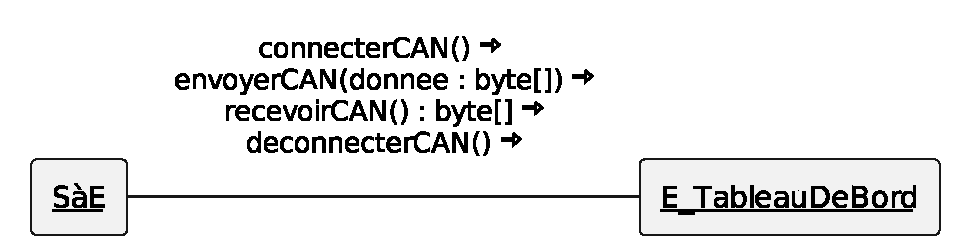
\includegraphics[width=14cm]{../schemas/contexte_phy}
    % \captionsetup{justification=centering}
    \caption{Contexte physique représenté \\par un diagramme de déploiement UML}
    \label{schema_contexte_phy}
\end{figure}

\subparagraph{En provenance du SàE}
\mbox{}\\

\textbf{Vers E\_TableauDeBord :} \vspace{0.2cm} \\ %SUBSUBPARAGRAPHE !
\textbf{connecterCAN()} --- Le SàE se connecte au bus CAN. \\
\textbf{envoyerCAN(donnee : byte[])} --- Le SàE envoie une ou plusieurs trames sur le bus CAN. \\
\textbf{recevoirCAN() : byte[] }--- Le SàE récupère la ou les trames sortantes de Tableau de Bord sur le bus CAN.  \\
\textbf{deconnecterCAN()} --- Le SàE se déconnecte du bus CAN. \\

